% Options for packages loaded elsewhere
\PassOptionsToPackage{unicode}{hyperref}
\PassOptionsToPackage{hyphens}{url}
%
\documentclass[
]{book}
\usepackage{lmodern}
\usepackage{amsmath}
\usepackage{ifxetex,ifluatex}
\ifnum 0\ifxetex 1\fi\ifluatex 1\fi=0 % if pdftex
  \usepackage[T1]{fontenc}
  \usepackage[utf8]{inputenc}
  \usepackage{textcomp} % provide euro and other symbols
  \usepackage{amssymb}
\else % if luatex or xetex
  \usepackage{unicode-math}
  \defaultfontfeatures{Scale=MatchLowercase}
  \defaultfontfeatures[\rmfamily]{Ligatures=TeX,Scale=1}
\fi
% Use upquote if available, for straight quotes in verbatim environments
\IfFileExists{upquote.sty}{\usepackage{upquote}}{}
\IfFileExists{microtype.sty}{% use microtype if available
  \usepackage[]{microtype}
  \UseMicrotypeSet[protrusion]{basicmath} % disable protrusion for tt fonts
}{}
\makeatletter
\@ifundefined{KOMAClassName}{% if non-KOMA class
  \IfFileExists{parskip.sty}{%
    \usepackage{parskip}
  }{% else
    \setlength{\parindent}{0pt}
    \setlength{\parskip}{6pt plus 2pt minus 1pt}}
}{% if KOMA class
  \KOMAoptions{parskip=half}}
\makeatother
\usepackage{xcolor}
\IfFileExists{xurl.sty}{\usepackage{xurl}}{} % add URL line breaks if available
\IfFileExists{bookmark.sty}{\usepackage{bookmark}}{\usepackage{hyperref}}
\hypersetup{
  pdftitle={Data analysis using R for Psychology},
  pdfauthor={Alexander (Sasha) Pastukhov},
  hidelinks,
  pdfcreator={LaTeX via pandoc}}
\urlstyle{same} % disable monospaced font for URLs
\usepackage{longtable,booktabs}
% Correct order of tables after \paragraph or \subparagraph
\usepackage{etoolbox}
\makeatletter
\patchcmd\longtable{\par}{\if@noskipsec\mbox{}\fi\par}{}{}
\makeatother
% Allow footnotes in longtable head/foot
\IfFileExists{footnotehyper.sty}{\usepackage{footnotehyper}}{\usepackage{footnote}}
\makesavenoteenv{longtable}
\usepackage{graphicx}
\makeatletter
\def\maxwidth{\ifdim\Gin@nat@width>\linewidth\linewidth\else\Gin@nat@width\fi}
\def\maxheight{\ifdim\Gin@nat@height>\textheight\textheight\else\Gin@nat@height\fi}
\makeatother
% Scale images if necessary, so that they will not overflow the page
% margins by default, and it is still possible to overwrite the defaults
% using explicit options in \includegraphics[width, height, ...]{}
\setkeys{Gin}{width=\maxwidth,height=\maxheight,keepaspectratio}
% Set default figure placement to htbp
\makeatletter
\def\fps@figure{htbp}
\makeatother
\setlength{\emergencystretch}{3em} % prevent overfull lines
\providecommand{\tightlist}{%
  \setlength{\itemsep}{0pt}\setlength{\parskip}{0pt}}
\setcounter{secnumdepth}{5}
\usepackage{booktabs}
\ifluatex
  \usepackage{selnolig}  % disable illegal ligatures
\fi
\usepackage[]{natbib}
\bibliographystyle{apalike}

\title{Data analysis using R for Psychology}
\author{Alexander (Sasha) Pastukhov}
\date{2020-10-29}

\begin{document}
\maketitle

{
\setcounter{tocdepth}{1}
\tableofcontents
}
\hypertarget{introduction}{%
\chapter*{Introduction}\label{introduction}}
\addcontentsline{toc}{chapter}{Introduction}

\hypertarget{about-the-seminar}{%
\section*{About the seminar}\label{about-the-seminar}}
\addcontentsline{toc}{section}{About the seminar}

This is a material for \emph{Applied data analysis for psychology using the open-source software R} seminar. Each chapter covers a single seminar, introducing necessary ideas and is accompanied by a notebook with exercises, which you need to complete and submit. The material assumes no foreknowledge of R or programming in general from the reader. Its purpose is to gradually build up your knowledge and introduce to a typical analysis pipeline. It is based on a data that is typical for the field (repeated measures, appearance, accuracy and response time measurements, Likert scale reports, etc.), you are welcome to suggest your own data set for analysis. Even if you already performed the analysis using some other program, it would still be insightful to compare the different ways and, perhaps, you might gain a new insight. Plus, it is more engaging to work on your data.

Remember that throughout the seminar you can and should(!) always ask me whenever something is unclear, you do not understand a concept or logic behind certain code. Do not hesitate to write me in the team or (better) directly to me in the chat (in the latter case, the notifications are harder miss and we don't spam others with our conversation).

You will need to submit your assignment one day before the next seminar (Tuesday before noon at the latest), so I would have time evaluate it and provide feedback.

As a final assignment, you will need to program a full analysis pipi line for a given data set (or, if you want, for your data set). All the necessary steps will be covered by the seminar material. Please inform me, If you require a grade, as then I will create a more specific description for you to have a clear understanding of how the program will be graded.

\hypertarget{note-on-exercises}{%
\section*{Note on exercises}\label{note-on-exercises}}
\addcontentsline{toc}{section}{Note on exercises}

In many exercises your will be not writing the code but understanding it. Your job in this case is ``to think like a computer''. Your advantage is that computers are very dumb, so instructions for them must be written in very simple, clear, and unambiguous way. This means that, with practice, reading code is easy for a human (well, reading a well-written code is easy, you will eventually encounter ``spagetti-code'' which is easier to rewrite from scratch than to understand). In each case, you simply go line-by-line, doing all computations by hand and writing down values stored in the variables (if there are too many to keep track of). Once you go through code in this manner, it will be completely transparent for you. No mysteries should remain, you should have no doubts or uncertainty about any(!) line. Moreover, then you can run the code and check that the values you are getting from computer match yours. Any difference means you made a mistake and code is working differently from how you think it does. In any case, \textbf{if you not 100\% sure about any line of code, ask me, so we can go through it together!}

In a sense, this is the most important programming skill. It is impossible to learn how to write, if you cannot read first! Moreover, when programming you will probably spend more time reading the code and making sure that it works correctly than writing the new code. Thus, use this opportunity to practice and never use the code that you do not understand completely. So do use \href{https://stackoverflow.com/}{stackoverflow} but do make sure you understand the code you copied!

\hypertarget{why-r}{%
\section*{Why R?}\label{why-r}}
\addcontentsline{toc}{section}{Why R?}

There are many software tools that allow you preprocess, plot, and analyse your data. Some cost money (SPSS, Matlab), some are free (Python, Julia) just like R. Moreover, you can replicate all the analysis that we will perform using Python in combination with \href{https://jupyter.org/}{Jupyter notebooks} (for reproducable analysis), \href{https://pandas.pydata.org/}{Pandas} (for Excel-style table) and \href{https://www.statsmodels.org/stable/index.html}{statmodels} (for statistical analysis). However, R in combination with \href{https://www.tidyverse.org/}{Tidyverse} family of packages is optimized for data analysis pipeline, making it easy to write simple, powerful and expressive code that is very easy to understand (a huge plus, as you will discover). I will run circles around myself trying to replicate the same analysis in Python or Matlab. In addition, R is loved by mathematicians and statisticians, so it tends to have implementations for all cutting edge methods (my impression is that even Python is lagging behind it in that respect).

\hypertarget{tidyverse-versus-base-r}{%
\section*{Tidyverse versus base R}\label{tidyverse-versus-base-r}}
\addcontentsline{toc}{section}{Tidyverse versus base R}

I will be teaching what one might call a ``dialect'' of R, based on \href{https://www.tidyverse.org/}{Tidyverse} family of packages. R is extremely flexible,making it possible to redefine its own syntax. Because of that Tidyverse-based code will look very different from the base R code to the point that it might look like written in two completely different languages (which, in a sense, it is). Although Tidyverse, at least in my opinion, is a better way, we will start with \emph{base R}, so that you will be able to read and understand code written outside of Tidyverse, as it is also very common.

\hypertarget{getting-started}{%
\chapter*{Getting Started}\label{getting-started}}
\addcontentsline{toc}{chapter}{Getting Started}

\hypertarget{installing-r}{%
\section*{Installing R}\label{installing-r}}
\addcontentsline{toc}{section}{Installing R}

Go to \href{https://cloud.r-project.org/}{r-project.org} and download the current stable version of R for your platform. Run the installer, accepting all defaults. The installer will ask you whether you also want the 32-bit version to be installed alongside 64-bit. You probably won't need 32-bit, so if space is at premium you can skip it. Otherwise, it will make very little difference.

\hypertarget{installing-r-studio}{%
\section*{Installing R-Studio}\label{installing-r-studio}}
\addcontentsline{toc}{section}{Installing R-Studio}

Go to \href{https://rstudio.com/products/rstudio/download/}{rstudio.com} and download \emph{RStudio Desktop Free} edition for your platform. Install it using defaults. The \emph{R-Studio} is an integrated development environment for R but you need to install R separately first! The R-Studio will automatically detect latest R that you have and, in case you have several versions of R installed, you will be able to alter that choice.

I will explain the necessary details on using R-Studio throughout the seminar but the \href{https://github.com/rstudio/cheatsheets/raw/master/rstudio-ide.pdf}{official cheatsheet} is an excellent, compact, and up-to-date source of information. In fact, R Studio has numerous \href{https://rstudio.com/resources/cheatsheets/}{cheatsheets} that describe individual packages in a compact form.

\hypertarget{rtools}{%
\section*{Installing RTools}\label{rtools}}
\addcontentsline{toc}{section}{Installing RTools}

If you are using Windows, we might need \href{https://cran.r-project.org/bin/windows/Rtools/}{Rtools} for building and running some packages. You do not need to install it at the beginning, but when we will need it later, just following the link above, download the latest \emph{Rtools} version, run the installer using the defaults and \textbf{follow the instructions on that page to put Rtools on the PATH}! (I do not repeat them here, because they might change).

\hypertarget{installing-packages}{%
\section*{Installing packages}\label{installing-packages}}
\addcontentsline{toc}{section}{Installing packages}

The real power of R lies in a community-driven vast family of packages suitable for any occasion. The default repository used by R and R-Studio is \href{https://cran.r-project.org/}{The Comprehensive R Archive Network} (a.k.a. \emph{CRAN}). It has very strict requirements for submitted packages, which makes it very annoying for the authors but ensures high quality of most packages, as they tend to be well-documented and come with example data and code. We will use CRAN as a sole source for packages, but there are alternatives, such as \href{http://www.bioconductor.org/}{Bioconductor} that might have a package that is missing at CRAN. The Bioconductor relies on its own package manager, so you will need to consult latest manual on their website.

To install CRAN package you have two alternatives: via command line function or via R-Studio package manager interface. In the former case, go to \texttt{Console} tab and type \texttt{install.packages("package-name")}, for example \texttt{install.packages("tidyverse")}, and press \texttt{Enter}.

\begin{center}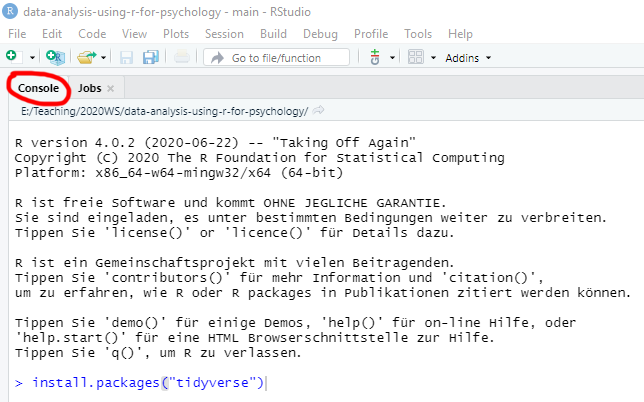
\includegraphics[width=1\linewidth]{images/install-packages-cmd} \end{center}

Alternatively, go to \texttt{Packages} tab, click on \texttt{Install} button, enter the package name in the window, which has autocomplete to help you, and press \texttt{Install}.

\begin{center}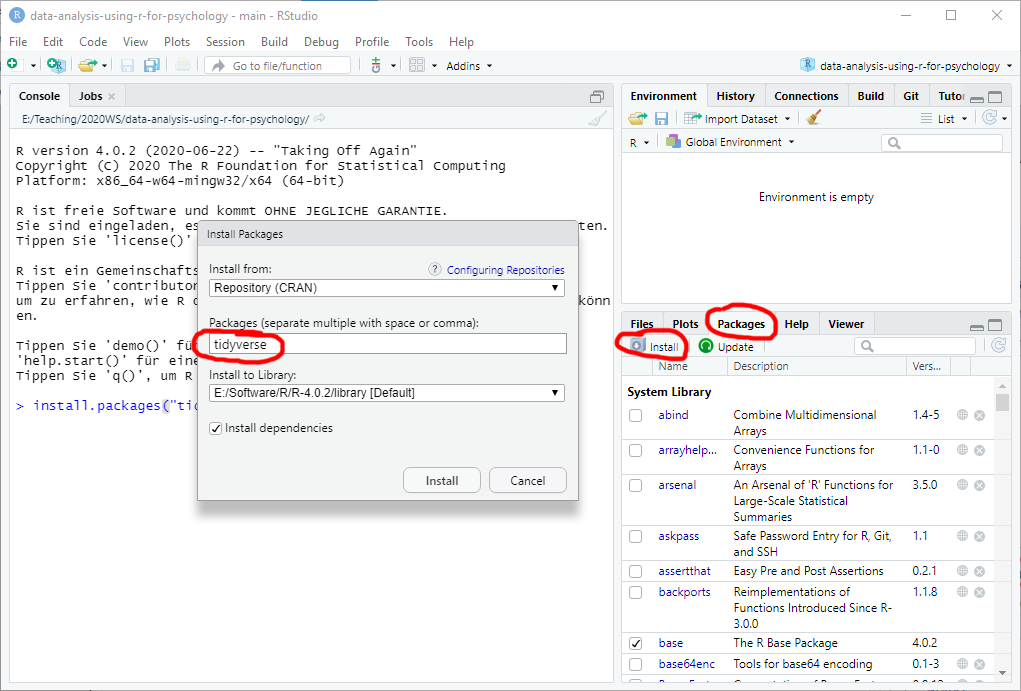
\includegraphics[width=1\linewidth]{images/install-packages-gui} \end{center}

In some cases, R will ask whether you want to install packages from source. In this case, it will grab the source code and compile the package, which takes time and requires \protect\hyperlink{rtools}{RTools}. In most cases, you can say ``No'' to install a pre-build binary version. The binary version will be slightly outdated but the emphasis is on \emph{slightly}.

Please install the following packages:

\begin{itemize}
\tightlist
\item
  \texttt{tidyverse} : includes packages from data creation (\texttt{tibble}), reading (\texttt{readr}), wrangling (\texttt{dplyr}, \texttt{tidyr}), plotting (\texttt{ggplot2}). Plus type specific packages (\texttt{stringr} for strings, \texttt{forcats} for factors) and functional programming (\texttt{purrr}).
\item
  \texttt{rmarkdown} : package for working with RMarkdown notebooks, which will we use to create reproducible analysis.
\item
  \texttt{fs} : file system utilities.
\end{itemize}

\hypertarget{keeping-r-and-packages-up-to-date}{%
\section*{Keeping R and packages up-to-date}\label{keeping-r-and-packages-up-to-date}}
\addcontentsline{toc}{section}{Keeping R and packages up-to-date}

R and packages are getting constantly improved, so it is a good idea to regularly update them. For packages, you can use \texttt{Tools\ /\ Check\ for\ Packages\ Updates...} menu in R-Studio. To update R and, optionally, packages, you can use \href{https://www.r-project.org/nosvn/pandoc/installr.html}{installr} package that can install newest R (but it keeps old version!) optionally copying your entire library of packages, update packages, etc. For R-Studio itself, use \texttt{Help\ /\ Check\ for\ Updates} menu and install a newer version, if it is available (it is generally a good idea to keep your R-Studio in the newest state).

\hypertarget{reproducable-research}{%
\chapter*{Reproducable Research and RMarkdown Notebooks}\label{reproducable-research}}
\addcontentsline{toc}{chapter}{Reproducable Research and RMarkdown Notebooks}

  \bibliography{book.bib}

\end{document}
